%!TEX root = Presentation-Thoma.tex
\section{Verfahren}
\subsection{Verfahren}

\begin{frame}{Sliding Window + Allgemeiner Klassifizierer}
    \begin{figure}[ht]
        \centering
        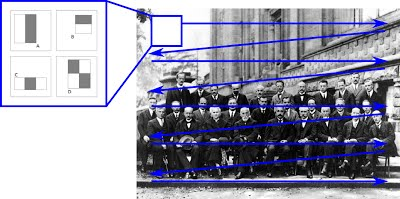
\includegraphics[width=\textwidth]{../images/sliding_window.jpg}
        \caption{\tiny \href{https://sites.google.com/site/5kk73gpu2012/assignment/viola-jones-face-detection}{sites.google.com/site/5kk73gpu2012/assignment/viola-jones-face-detection}}
        \label{fig:sliding-window}
    \end{figure}
\end{frame}

\begin{frame}{Features}
    \begin{figure}[ht]
        \centering
        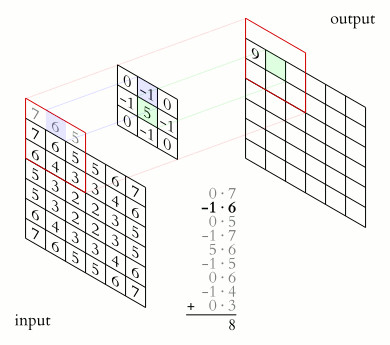
\includegraphics[height=0.8\textheight]{../images/kernel_convolution.jpg}
        \caption{\tiny \href{https://developer.apple.com/library/ios/documentation/Performance/Conceptual/vImage/Art/kernel_convolution.jpg}{developer.apple.com/library/ios/documentation/Performance/Conceptual/vImage/Art/kernel\_convolution.jpg}}
        \label{fig:conv}
    \end{figure}
\end{frame}

\begin{frame}{Features}
    \begin{itemize}
        \item Farbräume (RGB, HSV, LUV, XYZ, \dots)
        \item Histogram of Oriented Gradients (HOG)
        \item SIFT
        \item Bag-of-Visual-Words (BOV)
        \item Poselets
        \item Textons
        \item \dots
    \end{itemize}
\end{frame}

\begin{frame}{Random Forest}
    \begin{figure}[ht]
        \centering
        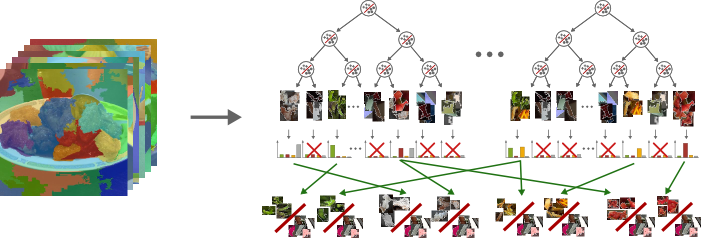
\includegraphics[width=\textwidth]{../images/rf-comp-mining.png}
        \caption{[Bossard et al. 2014]}
        \label{fig:input}
    \end{figure}

    \begin{itemize}[<+->]
        \item Ensemble von Entscheidungsbäumen (Decision Trees)
        \item Entscheidungsbäume sind Bäume für die Klassifikation
        \begin{itemize}
            \item Jeder innere Knoten trifft entspricht einer \texttt{if}-Abfrage.
            \item Jedes Blatt entspricht einem Label.
            \item \texttt{if}-Abfragen werden anhand der Features automatisch
                  generiert.
        \end{itemize}
    \end{itemize}
\end{frame}

\begin{frame}{Warum Random Forests?}
    \begin{columns}[t,onlytextwidth]
        \begin{column}{0.5\textwidth}
            \textbf{Vorteile}:
            \begin{itemize}
                \item Schneller Klassifikator
                \item Erklärbare Features
                \item Beliebige Skalen von Features (nominell, kategoriell, intervallskaliert, \dots)
                \item State-of-the-Art bei manchen Problemen
            \end{itemize}
        \end{column}
        \begin{column}{0.5\textwidth}
            \textbf{Nachteile}:
            \begin{itemize}
                \item Hand-Engineering der Features
                \item Nicht mehr State-of-the Art in Computer Vision
            \end{itemize}
        \end{column}
    \end{columns}
\end{frame}

\begin{frame}{Conditional Random Field}
    \includegraphics[width=\textwidth]{../images/graph-mrf-image-segmentation.pdf}
\end{frame}

\begin{frame}{Verfahren}
    \begin{itemize}
        \item \textbf{Sliding Window + Allgemeiner Klassifizierer}
        \begin{itemize}
            \item Random Forests
            \item SVMs
            \item Neuronale Netze
        \end{itemize}
        \item Markov Random Field / Conditional Random Field
        \item CNN + Tricks (vgl. Marvin)
    \end{itemize}
\end{frame}
